%----------------------------------------------------------------------------
\chapter{A részecskék detektálása}
%----------------------------------------------------------------------------

\section{Detektálási módszerek}
	A korábban látható \ref{fig:captures}. ábrán látható képeken kell a részecskéket felismerni és
	azoknak a koordinátáit exportálni.
	Erre több lehetőség adódik, amit a \cite{Feng2007} részletez.
	A detektáló módszereket a számítás igényeiknek növekvő sorrendjében mutatom be.
\subsection{Küszöb módszer}
	Legkézenfekvőbb módszer, hogy a kép pixeleinek világosságát összehasonlítjuk egy küszöb értékkel
	és ha az nagyobb ennél, akkor ezeket megjelöljük, mivel ott részecskét feltételezünk. 
	A módszer egyenletes háttér-világosság esetén jól működik és extra gyorsan számítható.
\subsection{Küszöb módszer szűréssel}
	A háttér világossága a \ref{fig:allo}. ábrán jól láthatóan nem egyenletes.
	A korábban említett egyszerű küszöb módszer itt nem alkalmazható, mivel a világos és sötét
	területek más és más küszöbértéket kívánnának meg.
	A megoldása erre, mint megannyi villamosmérnöki mérési feladatra, hogy a jel helyett a
	differenciális jelet mérjük. Jelen esetben ez azt jelenti, hogy először előállítjuk a részecske
	nélküli háttérképét, majd a méréssel kapott képből kivonva ezt a differenciális képet megkapjuk.
	A differenciális képen a részecskéket a korábban említett küszöb módszerrel lehet detektálni a
	részecskéket.
	
	Ehhez csupán a mérési képből kell szűréssel származtatni a háttérképet.
	A \cite{Feng2007,Oxtoby2010} cikkekben és általában erre véges Gauss szűrőt használnak, ami egy
	lineáris véges impulzusválaszú (FIR) aluláteresztő szűrő.
	A szűrés egy adott pixel környezetének súlyozott átlagolását jelenti.
	A súlyozás során szoroznunk kell, ami a bináris megvalósítás végett jóval lassabban történik, mint az
	összeadás avagy az összehasonlítás.
	
	Mivel a részecskék mérete a képen véges és kis szórású, így a korábban
	említett FIR Gauss szűrő jól tudja a részecskéket eliminálni.
	Viszont a mérési képek $100\ \mathrm{FPS}$ sebességgel és $1024\times1024$ mérettel érkeznek be.
	Ez $100\ \mathrm{MByte/s}$ adatfolyamot jelent. Ahhoz, hogy ezt közel real-time feltudjuk dolgozni
	a Gauss szűrés nem járható út. Hatékonyabb szűrőre van szükségünk! A megoldást a medián szűrőben látom,
	ami egy nemlineáris, de véges ``impulzusválaszú'' szűrő.
	A szűrő az adott pixel környezetének mediánjának számítását jelenti.
	A nemlinearitás jelen esetben nem okoz gondot, mivel csak detektálásra használjuk (a pozíció
	kinyerése az eredeti kép alapján készül, de ez később részletezve lesz.)
	
	A Gauss szűrő $n\times n$ környezet (ablak) esetén $n^2$ szorzást és $n^2-1$ összeadást jelent. Míg
	a medián szűrő $n\times n$ ablak esetén: bubborék rendezés során $O(n^2)$, javított bubborék
	rendezés során $O(n^2 / 2)$ illetve quicksort esetén $O(n\log n)$ összehasonlítást és
	cserét. Az összehasonlítás és a csere nagyságrendekkel gyorsabban végrehajtható, mint a szorzás és
	össeadás.
	
\subsection{Adaptív küszöb módszer szűréssel}
	Látható a \ref{fig:allo}. ábrán, hogy a sötétebb háttér kiterjedése nagyobb, ennek megfelelően az
	automata kamera ezekre a területekre állítja be az expozíciót.
	Így a sötét területek részletesebbek, míg a világos területek részletszegények (túlexponáltak) lesznek.
	Számunkra ez azt jelenti, hogy a sötétebb területeken jobban megbízhatunk a részecskék képében,
	míg a világosabb területeknél nem.
	Ezt a döntési küszöb értékének adaptációját jelenti a háttér világosságához.
	Az adaptív küszöböt a következő kifejezéssel határoztam meg:
	\begin{multline}
		\label{eq:treshold}
		K = \mathrm{Mean}\{P-\mhat{M}P\}+\\
		  + \delta \cdot \mathrm{STD}\{P - \mhat{M}P\} \cdot 
		\left[ 1+ a \left(
			\frac{\mhat{M}P}{\max\left\{\mhat{M}P\right\} - \min\left\{\mhat{M}P\right\}}
			\right)^b
		\right]
	\end{multline}
	ahol $P$ az eredeti kép, $\mhat{M} P$ a medián szűrt kép, $\mathrm{Mean}\{\},\ \mathrm{STD}\{\}$ az
	átlag és a szórás számításának függvénye és a $a,b$ két alakparaméter.
	\footnote{Az adaptív dontést a mérési kép előzetes feldolgozásával is elérhettük volna,
	ha a Photoshop-ból ismert Curves tool-al módosítottunk volna rajta. A tool a képet egy nemlineáris
	fügvényen keresztül engedi át.}
	
	A \ref{fig:alg}. ábrán látható a detektálási algoritmus működése közben.
	A \ref{fig:alg1}. ábrán a mérési kép ($P$) látható kitöltött görbével, ami az \ref{fig:allo}. ábrán
	látható mérési kép $x=40$ sora.
	Piros görbével látható a medián szűrt jelet ($\mhat{M}P$), amin jól érzékelhető a hirtelen
	változások eliminációja.
	A következő \ref{fig:alg2}. ábrán az eredeti és a szűrt különbsége azaz a differenciális kép
	($\partial P$) látható a kék görbével. A zöld görbe a \eqref{treshold} szerinti
	döntési köszöb.
	Az utolsó \ref{fig:alg3}. ábrán a detektált részecskék figyelhetőek meg.
	
	\begin{figure}[!h]
		\centering
		\subfloat[Eredeti (kitöltött) és a medián szűrt (folytonos) jel]{
			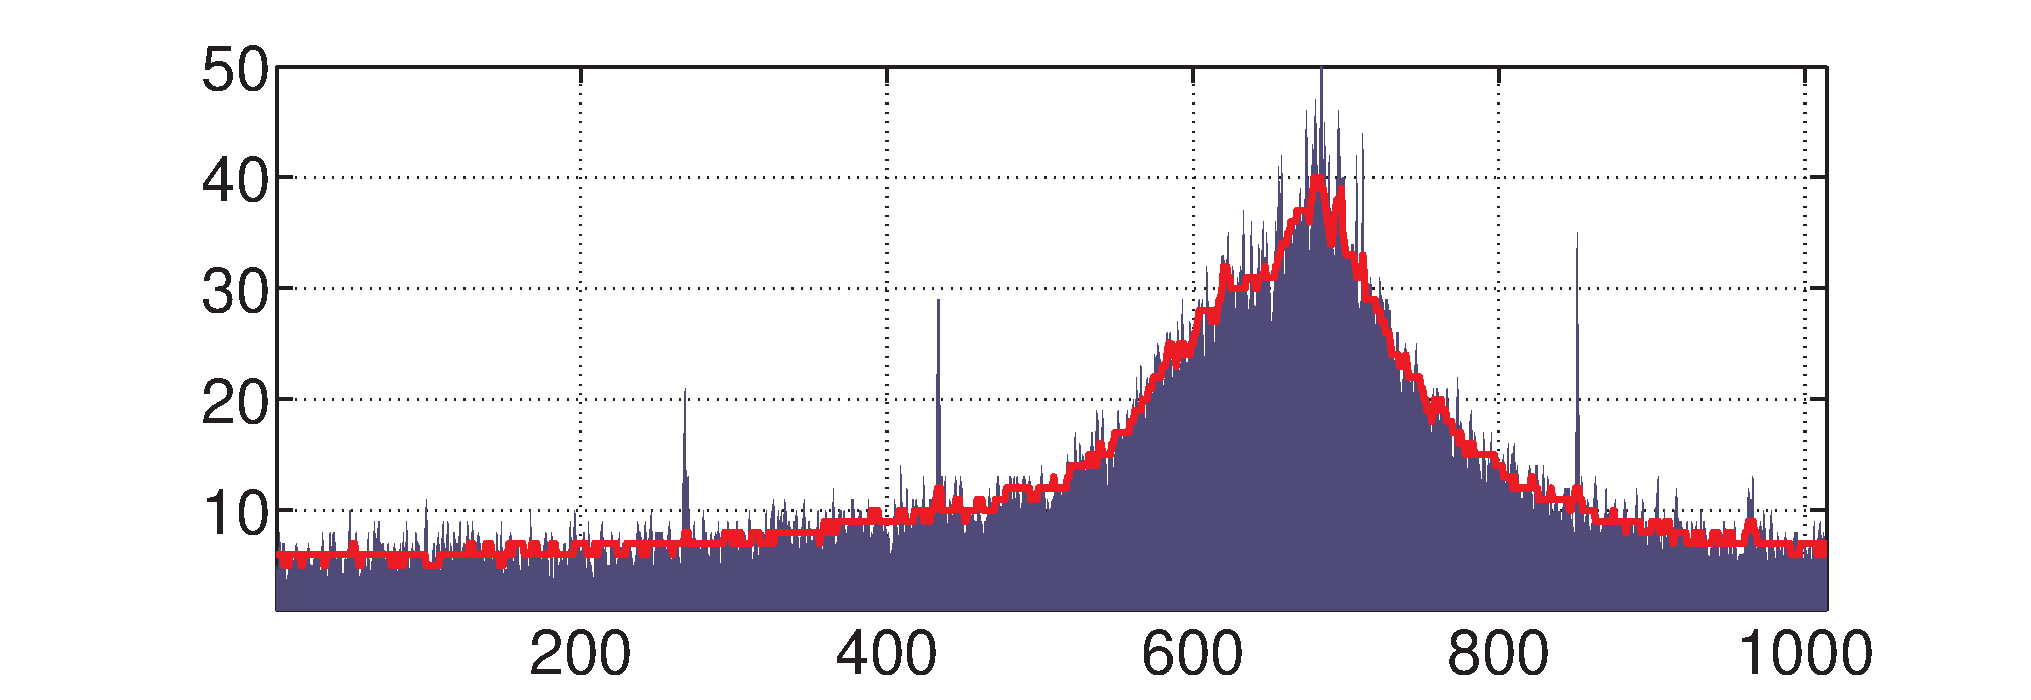
\includegraphics[width=0.95\columnwidth]{figures/eps/algoritmus1.eps}%
			\label{fig:alg1}
		}
		\\
		\subfloat[A differenciális jel (kék) és a döntési küszöb (zöld)]{
			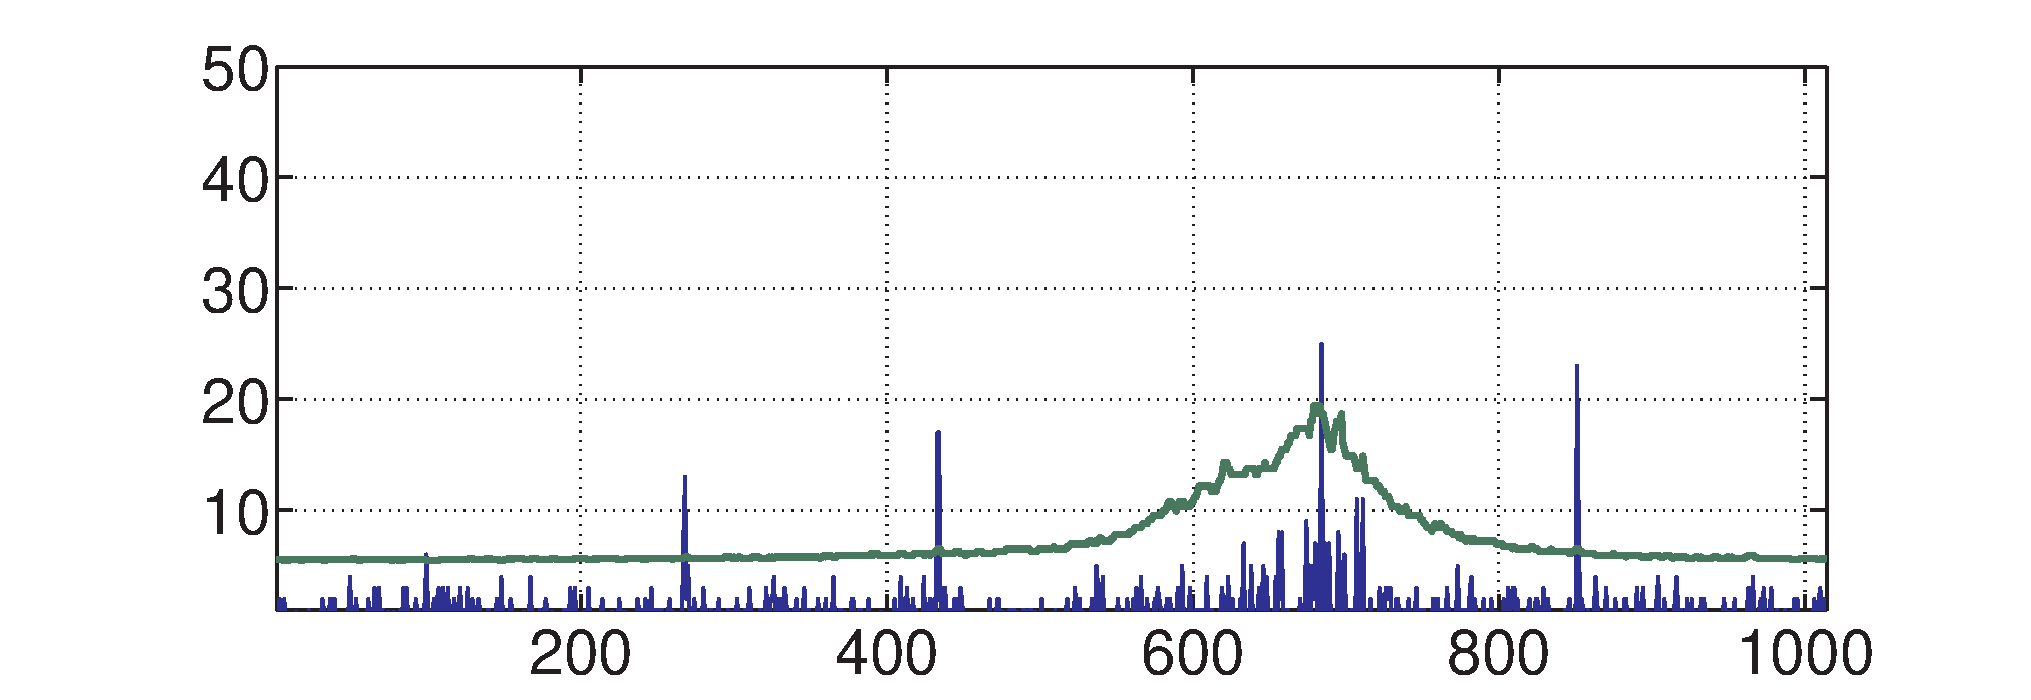
\includegraphics[width=0.95\columnwidth]{figures/eps/algoritmus2.eps}%
			\label{fig:alg2}
		}
		\\
		\subfloat[Detektált részecskék]{
			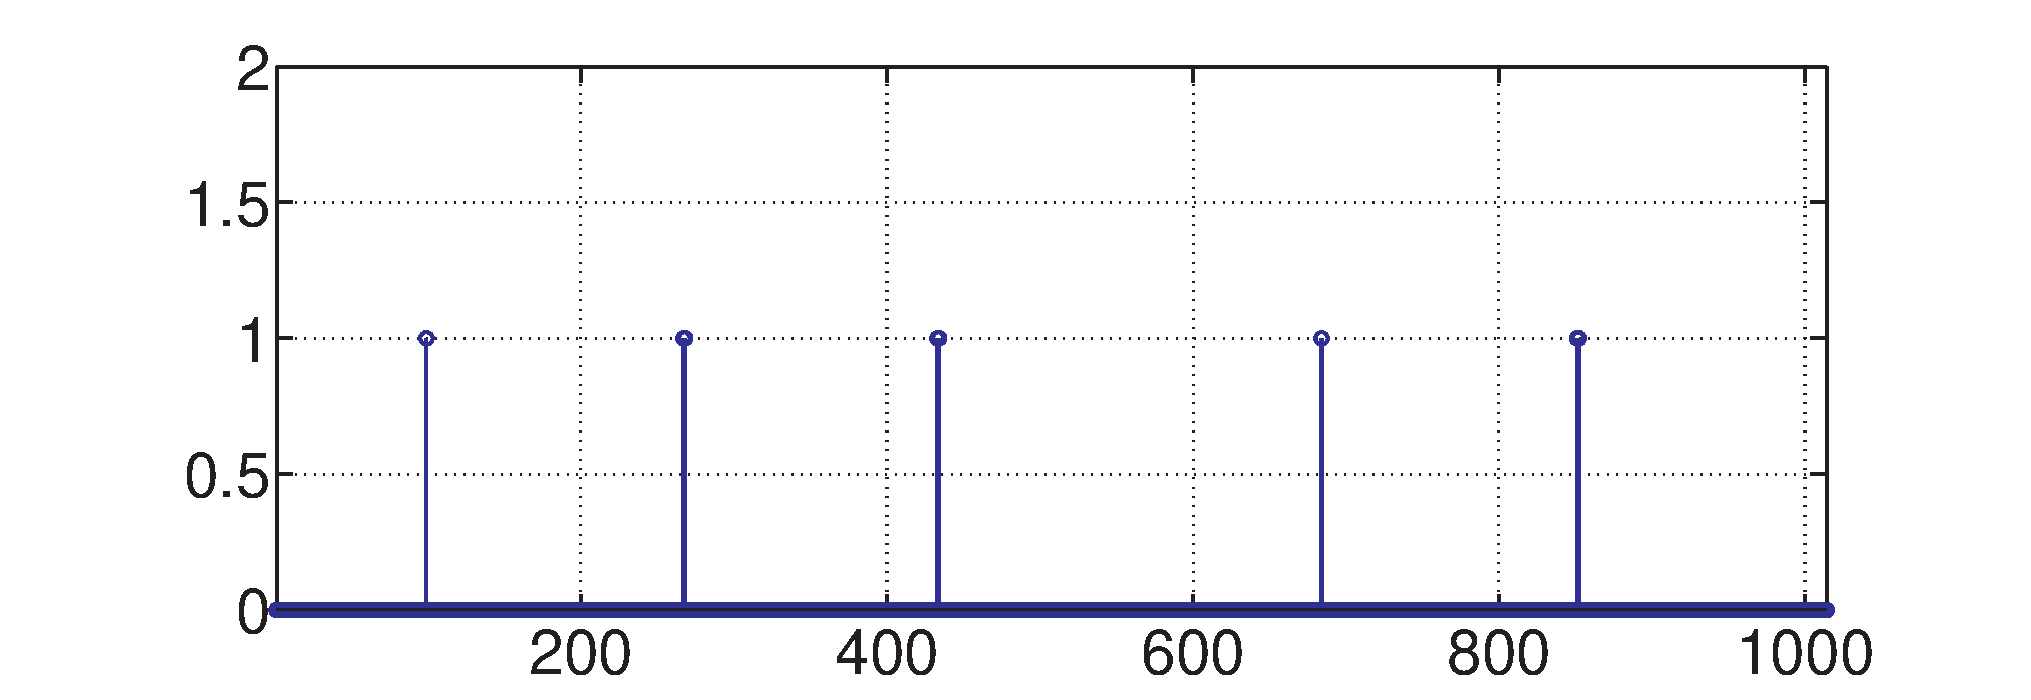
\includegraphics[width=0.95\columnwidth]{figures/eps/algoritmus3.eps}%
			\label{fig:alg3}
		}
		\caption[Adaptív küszöb bemutatása]{A medián szűrést alkalmazó adaptív küszöbbel részecskét
		detektáló algoritmus bemutatása az álló mérési kép (\ref{fig:allo}. ábra) $x=40$ során.}
		\label{fig:alg}
	\end{figure}
	
\section{A részecskék pozíciójának számítása}
	Kis felbontású kamera illetve nagyon kis porrészecskék esetén előállhat, hogy a részecskék egy
	pixelnyi területet foglalnak el a képen. Detektálás szempontjából ez kedvező viszont a pozíciómérés
	szempontjából nem, mivel ilyenkor a felbontásunk 1 pixelnyi. Ezen javítani a dithereléssel a
	következőképpen lehet: picit elállítjuk az élességet úgy, hogy egy részecske több pixel nagyságú
	``maszat'' legyen, majd a korábban részletezett detektálást elvégezzük.
	
	Ennek hatására egy részecske több pixelnyi felületet fog elfoglalni és a detektáló algiritmus is
	több pixelt fog megjelölni. A pozíció megtalálásához csoportosítani kell a megjelölt pixeleket.
	Az egy részecskéhez tartozó pixel-csoportot egy téglalap fogja határolni, amit region of
	interest-el (ROI) szokás illetni. Azonban a részecske detektálása után amorf formájú megjelölt
	pixeleink lesznek. Ezeket a könnyebb csoportosítás végett kiterjesztem pár pixellel az így kapott
	képet flood-fill algorimussal egybefüggővé teszem és ennek eredményeképp megkapom a ROI határoló
	koordiánáit, amit a következő két módszer felhasznál a részecske pozíciójának számítása során.
	\subsection*{Maximum keresés}
	Legegyszerűbb eset, ha a ROI-n belül az eredeti pixelek közül a legvilágosabbat veszem a
	részecske pozíciójaként.
	\subsection*{Szubpixel felbontás momentum módszerrel}
	Szofisztikáltabb, ha a ROI-n belül az eredeti pixelek világosságát, mint tömegpont tömegének veszem
	és a ROI-által határolt test súlypontját megkeresem. A módszerre kritikusan hat az előbb említett
	kiterjesztés mértéke. Ha túl nagy a kiterjesztés, akkor azzal hibát viszek be pozicíó mérésébe,
	míg ha túl kicsi akkor meg egy részecskének akár két képe/pozíciója keletkezhet.
	
	\noindent Az algoritmus hatékonyságát különböző $\delta$ érték mellett a következő \figref{roi}
	ábrán látható.
	
	\begin{figure}[H]
		\centering
		\subfloat[$\delta = 10$]{
			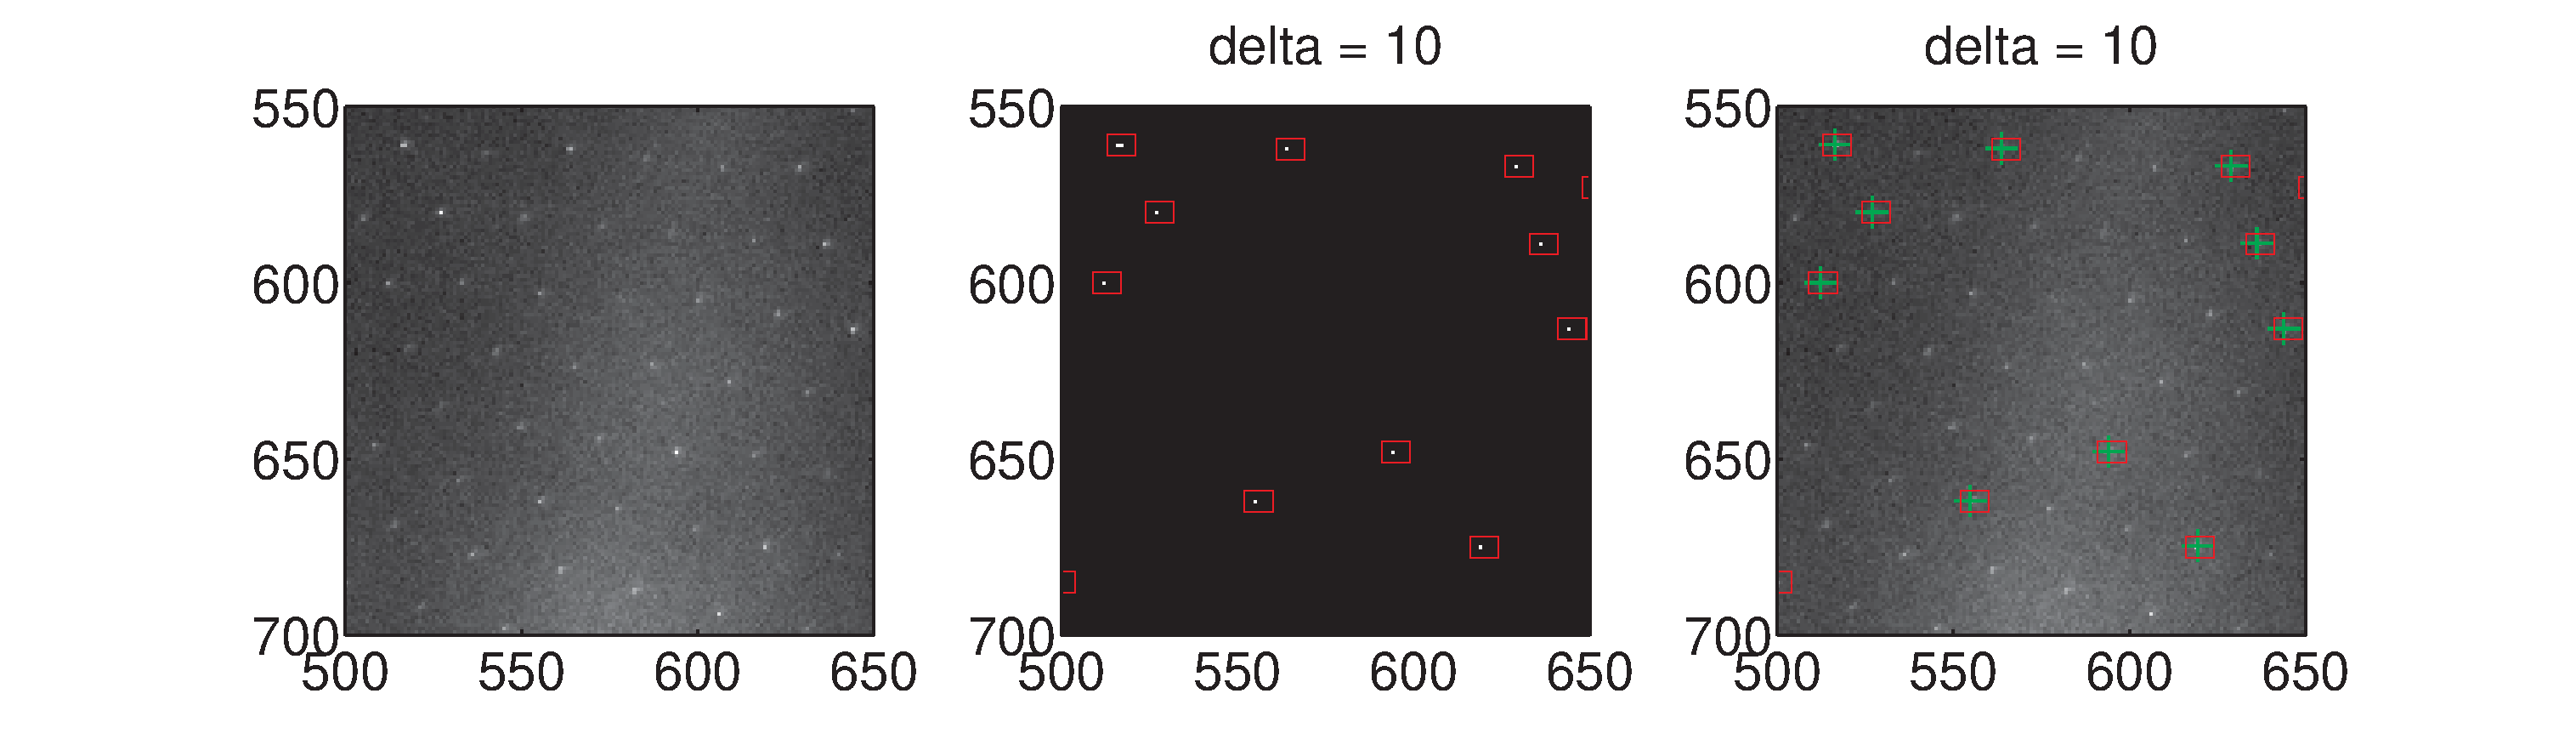
\includegraphics[width=1\columnwidth]{figures/eps/delta10.eps}%
			\label{fig:delta4}
		}
		\\
		\subfloat[$\delta = 2$]{
			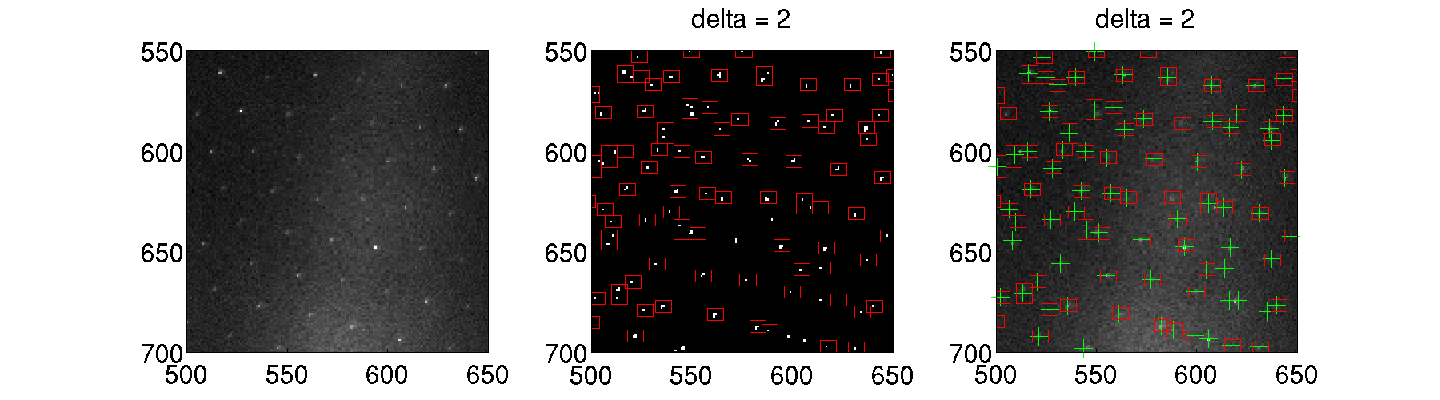
\includegraphics[width=1\columnwidth]{figures/eps/delta2.eps}%
			\label{fig:alg3}
		}
		\\
		\subfloat[Optimális $\delta = 3.5$]{
			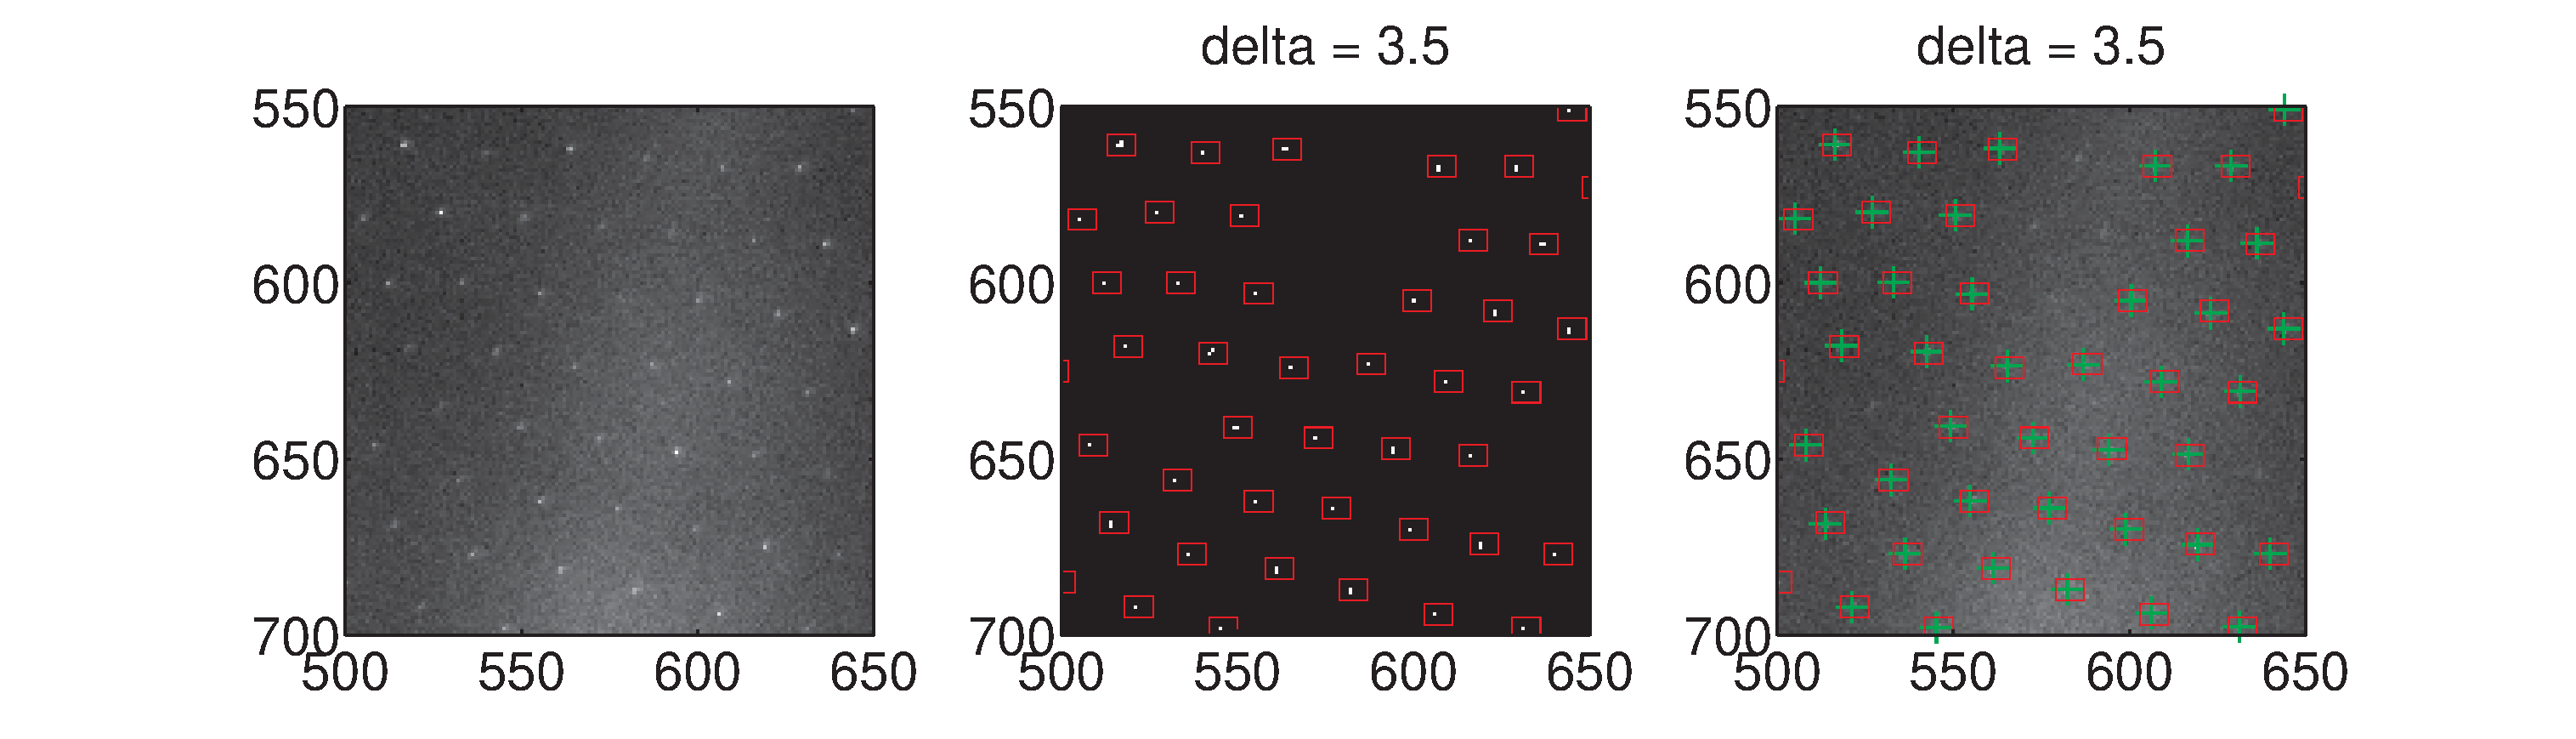
\includegraphics[width=1\columnwidth]{figures/eps/deltaopt.eps}%
			\label{fig:deltaopt}
		}
		\caption[Pozíciómérés momentum módszerrel]{Az adaptív küszöb módszerrel detektált részecskék
		momentum módszerrel számított pozíciója. \textbf{Bal oszlopban} az eredeti mérési kép, \textbf{középső oszlopban} a detektálás
		eredménye és a ROI, az \textbf{utolsó oszlopban} az eredeti mérési képen a ROI és a detektált
		részecske pozícióját jelző kereszt.}
		\label{fig:roi}
	\end{figure}
	
	\noindent
	\begin{center}
	Az algoritmus jól párhuzamosítható, ami a nagyteljesítményű multiprocesszoros
	környezetben kedvező futási időt eredményezhet. A párhuzamos program létrehozásának segítségére az 
	OpenCL keretrendszert választottam, aminek a bemutatása következik.
	\end{center}





